\documentclass[10pt]{jarticle}
\usepackage{float}
\usepackage{adrobo_abst}
\usepackage[dvipdfmx]{graphicx}
\usepackage{amssymb,amsmath}
\usepackage{bm}
\usepackage[superscript]{cite}
\usepackage{enumerate}
\usepackage{url}
%\usepackage[absolute]{textpos}

\renewcommand\citeform[1]{(#1)}

\begin{document}
    
    \makeatletter
    \doctype{2022年度卒業論文概要}
    \title{視覚と行動のend-to-end学習により経路追従行動を\\オンラインで模倣する手法の提案}{(目標方向による経路選択機能の追加と検証)}
    \etitle{A proposal for an online imitation method of path-tracking
    behavior by end-to-end learning of vision and action}{(Addition and verification of path selection function by target direction)}
    
    \author{19C1101\hspace{.5zw}藤原柾}
    \eauthor{Masaki FUJIWARA}
    
    \makeatother
    
    \abstract{An end-to-end learning approach leveraging camera images has been explored as a novel option for robotic navigation. To enable the robot to control the trajectory it takes at junction points, we introduce a path selection function. To this end, we propose a method to incorporate a target direction into the dataset of the preceding technique. The suggested procedure is subdivided into two stages: a learning stage and an evaluation stage. The efficacy of the proposed technique was validated in both a simulated and a real environment. Moreover, we addressed the issue of learning time.}
    
    \keywords{End-to-end learning, Navigation, Target direction}
    
    \maketitle
    
    \supervisor{指導教員:林原靖男 教授}
    
    \section{緒\hspace{2zw}言}
    
    近年, 機械学習を用いた自律走行の研究が進められている. Bojarski\cite{bojarski}らは, 人間が操作するステアリングの角度とカメラ画像を用いて, end-to-endで模倣学習することで自律走行する手法を提案した. さらに, 岡田ら\cite{okada}はLiDAR, オドメトリを入力としたルールベース制御器による経路追従行動を, カメラ画像を用いてend-to-endで模倣学習を行った. その結果, カメラ画像に基づいてロボットが学習した経路を周回可能であることが確認されている. 本研究では, 岡田ら\cite{okada}の研究(以下, 「従来手法」と称する)を元に, 分岐路で「直進」, 「左折」などのコマンドによる制御で, 経路を選択可能にする機能の追加を提案する. また, シミュレータ上での実験を実環境に移す際に, 問題となった学習時間の長さについて, 2 つのアプローチにより解決を図る. さらに, 実環境での提案手法の有効性を検証することを目的とする.
    
    \section{従来手法}
    岡田らの従来手法に関して紹介する. 
    \reffig{sample-fig}に, 経路追従行動を視覚に基づいてオンラインで模倣するシステムを示す. 
    手法は機械学習により, 学習器の訓練を行う「学習フェーズ」と訓練した結果を検証する「テストフェーズ」に分かれる.
    % \vspace{10pt}
    % \begin{center}
    %     \begin{figure}[!b]
    %         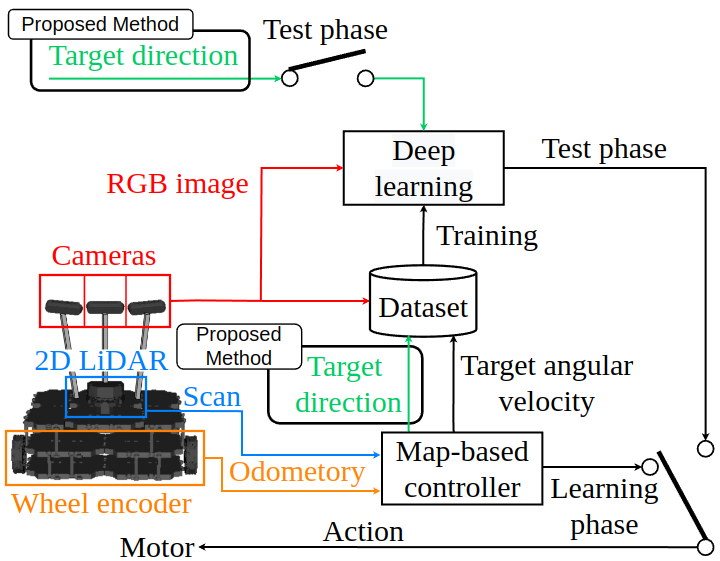
\includegraphics[width=0.45\textwidth]{./fig/system2.png}
    %         \caption{Imitation learning system}
    %         \label{fig:sample-fig}
    %     \end{figure}
    % \end{center}
    % \vspace{-0.5cm}
    \subsection{学習フェーズ}
    学習フェーズは, 模倣学習によって学習器の訓練を行うフェーズである. LiDARとオドメトリを入力とする地図を用いたルールベース制御器で自律走行する. この経路追従行動を, カメラ画像を用いたend-to-endで模倣学習する.

    \begin{center}
        \begin{figure}[h]
            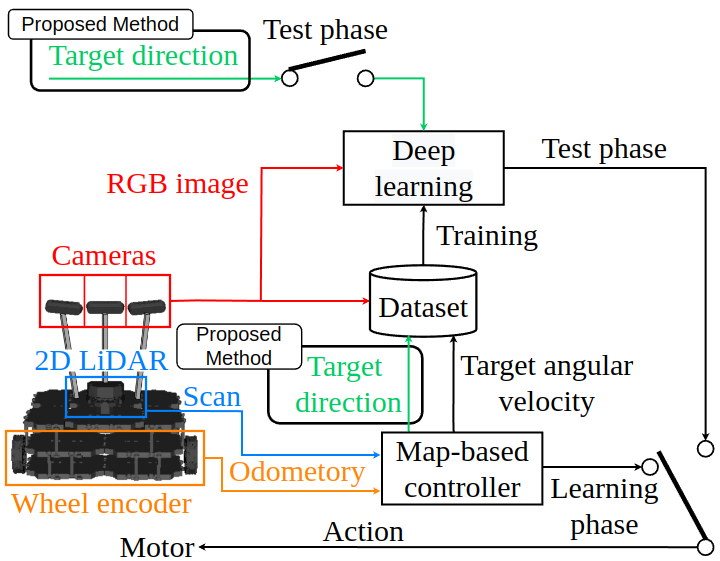
\includegraphics[width=0.45\textwidth]{./fig/system2.png}
            \caption{Imitation learning system}
            \label{fig:sample-fig}
        \end{figure}
    \end{center}

    \subsection{テストフェーズ}

    テストフェーズは, 訓練後の学習結果を評価するフェーズである. 学習器にカメラ画像を入力し, 出力されるヨー方向の角速度を用いて自律走行する.
    なお, \reffig{sample-fig}の提案手法と記載した部分は, 次章で述べるように, 本研究で追加した機能となる.

    \section{提案手法}

    経路選択機能の追加を目的として, データセットと学習器の入力へ「直進」, 「左折」などの目標方向を追加する. なお, 追加した要素以外は従来手法と同様である. \reffig{sample-fig}に, 提案手法のシステムを示す. 
    % なお, \reffig{sample-fig}では, 従来手法のシステムに追加した部分を提案手法と記載している. 
    学習フェーズでは, 目標方向の生成機能を追加した地図ベースの制御器を用いる. テストフェーズでは, 学習器の出力を用いた走行において, 目標方向によって任意の経路を選択する. 

    % \begin{center}
    %     \begin{figure}[h]
    %         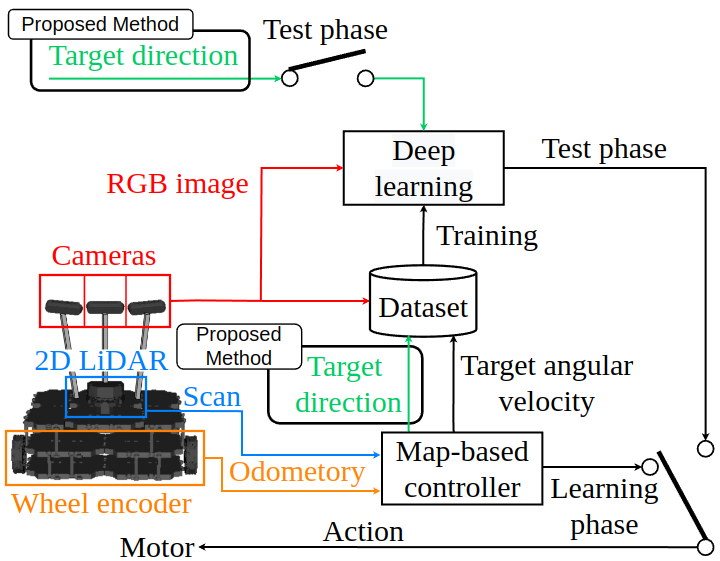
\includegraphics[width=0.45\textwidth]{./fig/system2.png}
    %         \caption{Sample of clear figure}
    %         \label{fig:propose_sys}
    %     \end{figure}
    % \end{center}

    本研究で用いた目標方向と学習器へ入力するデータ形式を, \reftab{target_direction}に示す. 目標方向は「直進(Go straight)」, 「左折(Turn left)」, 「右折(Turn right)」の3コマンドを用いる.
    \begin{table}[h]
        \caption{Target direction and data}
        \label{tab:target_direction}
        \begin{center}
            \vskip 1zh
            \begin{tabular}{|c|c|}
                \hline
                Target direction & Data \\ \hline
                Go straight & [100, 0, 0] \\ \hline
                Turn left & [0, 100, 0] \\ \hline
                Trun right & [0, 0, 100] \\ \hline
            \end{tabular}
        \end{center}
    \end{table}
    \vspace{-10pt}
    \section{実験}
    シミュレータ上での実験を実環境に移す際に問題となった学習時間の長さについて2つのアプローチを行い, 実験で有効性を確認する. また, 実環境での実験により, 提案手法の有効性を検証する.

    \subsection{実験内容}
    % 本稿では, 以下の2つの実験を行う.

    % \begin{enumerate}
    %     \item 2つのアプローチを行った実験
    % \end{enumerate}
    
    \begin{description}
        \item[実験1:2つのアプローチを行った実験]\mbox{}\\
        実験1では, 学習フェーズで予め決めた経路を繰り返し走行させる. その際に, コマンドのデータの偏りを減らすアプローチ1と, 蛇行走行するように制御指令を意図的に大きくするアプローチ2を行う. テストフェーズでは, 学習フェーズと同様の経路を, 目標方向による制御によって, 走行できるか評価を10回行う.
        \vspace{-10pt}
        \item[実験2:実環境での実験]\mbox{}\\
        実環境で実験1に倣って実験を行う.  
    \end{description}

    \subsection{実験装置}

    \begin{description}
        \item[実験1(シミュレータ)]\mbox{}\\
        ロボットは, \reffig{sample-fig}で示したような, Turtlebot3 waffle\_piへ3つのカメラを追加したモデルを用いる. また, シミュレータ上で千葉工業大学津田沼キャンパス2号館3階を模した環境を対象に実験を行う.
        \vspace{-10pt}
        \item[実験2(実環境)]\mbox{}\\
        % ロボットは, figに示すように, 3つのカメラを搭載したロボットを用いる. 
        実験は千葉工業大学津田沼キャンパス2号館3階で行った.
    \end{description}

    \subsection{実験結果}    
    各実験において, テストフェーズで正しい経路を選択できた成功率を\reftab{result}に示す. 
    
    実験1に関しては, 両方とも10000stepでアプローチを行わない場合と比べると, 成功率が向上している. また, 60000stepと20000stepで比べると, 成功率が悪化せずに学習step数を減らしている. 
    
    実験2に関しては, 成功率は65\%となり, シミュレータ上での実験結果より低くなった. 成功率が低い原因の解明には未だ至っていない. この問題の検討は, 今後の課題となっている. しかし, 経路選択前に同じ場所を走行し, ほぼ同様の画像が入力されている状態で, 目標方向に従って正しい経路を選択している様子を確認することができた.
    % このことから, 実環境においても提案手法により, 経路選択ができている可能性が高い.

    \begin{table}[h]
        \caption{Experimental results}
        \label{tab:result}
        \begin{center}
            \vskip 1zh
            \begin{tabular}{|c|c|c|}
                \hline
                Experimets & step & Success rate \\ \hline
                1 without approach & 60000 & 94.2\%\\ \hline
                1 without approach & 10000 & 72.5\%\\ \hline
                1 & 10000 & 90.8\%\\ \hline
                1 & 20000 & 95\%\\ \hline
                2 & 20000 & 65\%\\ \hline
                % Trun right & [0, 0, 100] \\ \hline
            \end{tabular}
        \end{center}
    \end{table}

    % \textbf{実験1}

    % \section{図及び写真・表の作成に関して}%===========================
    % \begin{enumerate}
    %     \setlength{\parskip}{0cm} % 段落間
    %     \setlength{\itemsep}{0cm} % 項目間
    %     \item 本文中では,\reffig{sample-fig},\reftab{sample-tab}のように日本語で書く.写真は,図として扱う.
    %     \item 番号・説明(キャプション)などは,図・写真についてはその下に,表についてはその上に書く.
    %     \item 本文と,図・表の間は1行以上の空白を空けて,見やすくする.
    %     \item 図中・表中の説明及びキャプションはすべて英語で書く(最初の文字は大文字とする).
    %     \item 図及び表がl列(片側)に収まらない場合2列(両側)にまたがって書くことができる. 
    %     \item 図及び表の横に空白ができても,その空白部には本文を記入してはならない.
    % \end{enumerate}
    
    % \begin{table}[t]
    %     \caption{Sample of expression of values}
    %     \label{tab:sample-tab}
    %     \begin{center}
    %         \vskip 1zh
    %         \begin{tabular}{|c|c|}
    %             \hline
    %             Recommend & Not recommend \\ \hline
    %             $0.357$ & $.357$ \\ \hline
    %             $3.141\ 6$ & $3.141,6$ \\ \hline
    %             $3.141\ 6 \times 2.5$ & $3.141\ 6 \cdot 2.5$ \\ \hline
    %         \end{tabular}
    %     \end{center}
    % \end{table}
    
    % \section{数式の書き方}%===========================
    
    % 式番号は,式と同じ行に右寄せして( )の中に書く.また,本文で式を引用するときは,\refeqn{sample-eq1}のように書く.
    % \begin{equation}
    %     \gamma(t) = \frac{ji}{N} \label{eq:sample-eq1}
    % \end{equation}
    % \begin{equation}
    % \bar{C}(t)=\frac{1}{N}\sum_{i=1}^{N}C_i(t) \label{eq:sample-eq2}
    % \end{equation}
    
    %\begin{table}[!b] \notag
    %\begin{minipage}{\textwidth}
    %\begin{tabular*}{\textwidth}{@{\extracolsep{\fill}}lr}
    %{\footnotesize
    %$\displaystyle 
    %u^*_{i,j} = u^n_{i,j} - \Delta t \left\{u^n_{i,j}\frac{u^n_{i+1,j} - u^n_{i-1,j}}{2\Delta x} + v^n_{i,j}\frac{u^n_{i,j+1} - u^n_{i,j-1}}{2\Delta y} + \frac{1}{Re}\left(\frac{u^n_{i+1,j} - 2u^n_{i,j} + u^n_{i-1,j}}{(\Delta x)^2} + \frac{u^n_{i,j+1} - 2u^n_{i,j} + u^n_{i,j-1}}{(\Delta y)^2}\right) \right\}
    %$}
    %& $\inlineTag\label{eq:long-eq} $
    %\end{tabular*}
    %\end{minipage}
    %\end{table}
    
    % 式を書くときは,2文字分空白を空ける.
    % また,必要行数分を必ず使うようにして書く.
    % 3行必要とする式を2行につめて書いたり,2行に分かれる式を1行に収めたりしない.
    % なお,本文と式,式相互間は1行以上の空白を空けて,見やすくする.
    % ポイント数は本文に準じるものとするが,添え字等が小さく読みにくくなるときは適宜拡大する.
    
    %式はなるべく片側に書くことが望ましいが,両側にまたがる場合は,読む順序に混乱を生じないように,そのページの式の上,または下の本文全部を両方にまたがるように書かなければならない.
    %本見本では\refeqn{long-eq}のようにページの最上段もしくは最下段に配置している場合は,上記のような混乱は生じ得ないので以下の文章は2段組で続けることができる.
    %ただし,所望の位置に表示されない,文字が重なるなどレイアウト上の多くの問題が生じるため,極めて推奨しない.
    
    % \section{引用文献の書き方}%===========================
    % 本文中の引用箇所には,右肩に小括弧をつけて,通し番号を付ける.例えば,文献\cite{工大2005}や,文献\cite{Shibutani2004, Handbook1979, Kikuchi2017, Adrobo2019}のようにする.
    
    % 引用文献は,英文で記述されているもの(文献\cite{Shibutani2004}など)は英文で書き,本文末尾に引用順にまとめて書く.専門的な書籍(文献\cite{Handbook1979}など)についても引用しても良い.
    % Web上の資料を引用する場合,例えばオンラインジャーナルなどの場合は文献\cite{Kikuchi2017}のように,webページの場合は文献\cite{Adrobo2019}のように,それぞれ参考文献として記載して引用する.この時,URLとともに参照日を記載すること.ただし,webページの場合は個人の技術ブログなどのように第3者による十分な審査が行われていないものの引用は行ってはいけない.公的な機関が発行しているページであっても,その永続性の問題から必要最小限に留めることを推奨する.
    % \vspace{-10pt}
        
    \section{結\hspace{2zw}言}%===========================
    
    % 本研究では, 経路追従行動をカメラ画像を用いた end-to-end 学習で模倣する岡田らの従来
    % 手法をベースに, データセットと学習器の入力へ目標方向を加えることで, 経路選択をする機
    % 能の追加を提案した. また, 
    シミュレータ上での実験を実環境に移す際に, 問題となった学習時
    間の長さについて, 2 つのアプローチを行うことで学習時間を大幅に削減した. 加えて, 実環
    境での実験を行い, 有効性の検証を行った. 実験結果より, 学習器へ目標方向を与えることで,
    指定した経路へ走行する挙動が確認できた.
    
    \vspace{5truemm}
    {\footnotesize
        \begin{thebibliography}{99}
            
            \bibitem{bojarski}
            Mariusz Bojarski et al: “End to End Learning for Self-
            Driving Cars”, 
            arXiv: 1604.07316,(2016)
            
            \bibitem{okada}
            岡田眞也, 清岡優祐, 上田隆一, 林原靖男: “視覚と行動のend-to-end 学習により経路追従行動 をオンラインで模倣する手法の提案”, 
            計測自動制御学会 si 部門講演会 sice-si2020予稿集,pp.1147–1152(2020).

        \end{thebibliography}
    }
    \normalsize
    
\end{document}
